\documentclass{article}

\usepackage{fancyhdr}
\usepackage{extramarks}
\usepackage{amsmath}
\usepackage{amsthm}
\usepackage{tikz}
\usepackage{enumerate}

\usetikzlibrary{automata, positioning}

\topmargin=-0.45in
\evensidemargin=0in
\oddsidemargin=0in
\textwidth=6.5in
\textheight=9.0in
\headsep=0.25in

\linespread{1.1}

\pagestyle{fancy}
\lhead{\hmwkAuthorName\ -\ \hmwkAuthorID}
\chead{\hmwkClass: Homework \hmwkNo}
\rhead{\firstxmark}
\lfoot{\lastxmark}
\cfoot{\thepage}

\renewcommand\headrulewidth{0.4pt}
\renewcommand\footrulewidth{0.4pt}

\newcommand{\enterProblemHeader}[1]{
    \nobreak\extramarks{}{Problem \arabic{#1} continued on next page\ldots}\nobreak{}
    \nobreak\extramarks{Problem \arabic{#1} (continued)}{Problem \arabic{#1} continued on next page\ldots}\nobreak{}
}

\newcommand{\exitProblemHeader}[1]{
    \nobreak\extramarks{Problem \arabic{#1} (continued)}{Problem \arabic{#1} continued on next page\ldots}\nobreak{}
    \stepcounter{#1}
    \nobreak\extramarks{Problem \arabic{#1}}{}\nobreak{}
}

\setcounter{secnumdepth}{0}
\newcounter{homeworkProblemCounter}
\setcounter{homeworkProblemCounter}{1}
\nobreak\extramarks{Problem \arabic{homeworkProblemCounter}}{}\nobreak{}

\newenvironment{homeworkProblem}[1][-1]{
    \ifnum#1>0
        \setcounter{homeworkProblemCounter}{#1}
    \fi
    \section{Problem \arabic{homeworkProblemCounter}}
    \enterProblemHeader{homeworkProblemCounter}
}{
    \exitProblemHeader{homeworkProblemCounter}
}


\newenvironment{solution}{
    \subsection{Solution}
}

\newcommand{\hmwkNo}{1}
\newcommand{\hmwkDueDate}{Sunday, March 17, 2019 at 11:59pm}
\newcommand{\hmwkClass}{CS244 Theory of Computation}
\newcommand{\hmwkClassInstructor}{Fu Song}
\newcommand{\hmwkAuthorName}{Name}
\newcommand{\hmwkAuthorID}{ID}

\title{
    \vspace{-0.4in}
    \textmd{\textbf{\hmwkClass \\ Homework \hmwkNo}}\\
    \normalsize\vspace{0.1in}\small{Due: \hmwkDueDate}\\
}

\author{\hmwkAuthorName\ -\ \hmwkAuthorID}
\date{}

\begin{document}

\maketitle
\thispagestyle{fancy}

You may discuss this assignment with other students and work
on the problems together. However, your write-up should be your own individual work and you should indicate in your submission who you worked with, if applicable. You should use the {\LaTeX} template provided by us to write your solution and submit the generated PDF file into Gradescope. \\

I worked with: (Name, ID), (Name, ID), \ldots \\

Let $\Sigma = \{\mathsf{0}, \mathsf{1}\}$ if not otherwise specified.

\begin{homeworkProblem}
Let $A$ be the set of all strings where there are no consecutive $\mathsf{0}$'s. Show that $A$ is regular in the following ways:
\begin{enumerate}[(a)]
    \item by giving an $\mathsf{NFA}$ that recognizes $A$,
    \item by giving a $\mathsf{DFA}$ that recognizes $A$,
    \item by giving a regular expression that describes $A$, and
    \item by giving a right linear grammar that describes $A$.
\end{enumerate}

\begin{solution}
\subsubsection{a)}
\subsubsection{b)}
	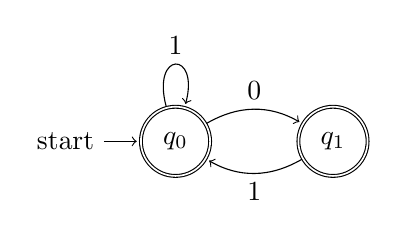
\begin{tikzpicture}[shorten >=1pt,node distance=2cm,on grid,auto]
		\node[state, initial, accepting] 	(q_0) 					{$q_0$};
		\node[state, accepting] 			(q_1) 	[right=of q_0] 	{$q_1$};
		\path[->]
			(q_0) 	edge 	[loop above] 	node 	{1} 	()
					edge 	[bend left]		node 	{0} 	(q_1)
			(q_1) 	edge 	[bend left]		node 	{1} 	(q_0);
	\end{tikzpicture}
\subsubsection{c)}
	\[
		L = 1^*(01^+)^*
	\]
\subsubsection{d)}
	$$ G = (\mathcal{N}, \Sigma, \mathcal{P}, \mathcal{S}) \texttt{ s.t. } \mathcal{N}=\{\mathcal{S}, A, B\}, \Sigma = \{0, 1\}, \mathcal{P} \texttt{ consists of the following rules: } $$
	\begin{equation*}\begin{aligned}
		& \mathcal{S} \rightarrow AB \\
		& A \rightarrow 1A | \epsilon \\
		& B \rightarrow 01A | \epsilon
	\end{aligned}\end{equation*}
\end{solution}

\end{homeworkProblem}

\begin{homeworkProblem}
Let $B$ be the set of all strings with even length that contain at least one $\mathsf{1}$ in their first half.
\begin{enumerate}[(a)]
    \item Show that $B$ is not regular.
    \item Show that $B$ is context free.
\end{enumerate}
\begin{solution}
\subsubsection{a)}
	\begin{proof}
		Let's proof by contradiction: Suppose $B$ is regular, is must satisfy pumping lemma, then $\exists p \ge 1$ \\
		Now consider string $0^{2p-1}10^{2p} \in B$. \\
		To satisify condition 3: $|xy| \le q$, it is safe to say that $x=0^s$, $y=0^t$ and $t > 0$ and $s + t \le p$. \\
		Then $\forall i$, $xy^i=0^{s+ti}$, $xy^iz = 0^{s+ti+(2p-1-s-t)}10^{2p}$. \\
		To fail condition 1, we can have $xy^i$ long enough to fail condition "at lease one $\mathsf{1}$ in the first half" and formulate the following equation:
		\begin{equation*}\begin{aligned}
			 |xy^i| &\ge \frac{1}{2}(|xy^iz|) \\
			 s + it &\ge \frac{1}{2}(s + ti + 2p-1-s-t + 1 + 2p) \\
			 i 		&\ge \frac{1}{t}(4p-2s-t) > 1
		\end{aligned}\end{equation*}
		Therefore, $\forall i \ge \frac{1}{t}(4p-2s-t)$, condition 1 cannot stand, this contradicts to pumping lemma which claims that $\forall i$, condition 1 stand. \\
		Therefore, we  claim that $B$ is not regular.
	\end{proof}
\subsubsection{b)}
\end{solution}
\end{homeworkProblem}

\begin{homeworkProblem}
Show that the following languages are not regular. B refers to the language in Problem 2.
\begin{enumerate}[(a)]
    \item $C = \{w \mid w \in B \text{ or } w \text{ has odd length}\}$.
    \item $D = \{w \mid w \text{ has even length but } w \notin B\}$.
\end{enumerate}
\end{homeworkProblem}
\begin{solution}
\subsubsection{b)}
	\begin{proof}
		Let's rephrase $D$ first. $D = \{lr | l=0^k, r = \Sigma^k\}$, that is to say, $\forall s \in D$, there is no $\mathsf{1}$ in the fist half $s$
		\\
		We would be proofing that $D$ is not regular by using Myhill-Nerode Theorem. \\
		Consider an infinite array of strings: $s_k = 0^k1, k = 1, 2, 3, \cdots$, we would be proving that they are not equivalent to each other w.s.t. $\~_L$ \\
		\\
		$\forall i \ne j$, without loss of generation, let's assume $i > j$. \\
		Then we can construct a $u = 1^j$ s.t. $s_ju \in D$ yet $s_iu \notin D$ \\
		\\
		Therefore, we proved that $D$ is not regular by proving that $D$ has a equivalent class that has infinite size.
	\end{proof}
\end{solution}

\begin{homeworkProblem}
For any string $w = w_1 w_2 \dotso w_n$, the \emph{reverse} of $w$, written as $w^\mathcal{R}$, is the string $w$ in reverse order, $w_n \dotso w_2 w_1$. For any language $A$, let $A^\mathcal{R} = \{w^\mathcal{R} \mid w \in A\}$. Show that if $A$ is regular, so is $A^\mathcal{R}$, i.e., regular languages are closed under reversal.
\end{homeworkProblem}

\begin{homeworkProblem}
Consider the following $\mathsf{CFG}\ G$:
$$S \to \mathsf{0} S \mathsf{1} \mid \mathsf{00} S \mathsf{1} \mid \varepsilon$$
Describe $L(G)$ and show that $G$ is ambiguous. Give an unambiguous grammar $H$ where $L(H) = L(G)$ and sketch a proof that $H$ is unambiguous.
\end{homeworkProblem}
\begin{solution}
\subsubsection{a)}
	$$L(G) = \{0^i1^j | i=x+y, j=x+2y\}$$
\end{solution}

\begin{homeworkProblem}
Let $E = \{rst \mid r, t \in \mathsf{0}^* \text{ and } s \in \mathsf{0}^* \mathsf{1} \mathsf{0}^* \text{ where } |r| = |s| = |t|\}$. Show that $E$ is context free in two ways:
\begin{enumerate}[(a)]
    \item by giving a $\mathsf{CFG}$ that generates $E$, and
    \item by giving a $\mathsf{PDA}$ that recognizes $E$.
\end{enumerate}
\end{homeworkProblem}

\begin{homeworkProblem}
Let $F = \{rst \mid r, s, t \in \mathsf{0}^* \mathsf{1} \mathsf{0}^* \text{ where } |r| = |s| = |t|\}$.
\begin{enumerate}[(a)]
    \item Show that $F$ is not context free.
    \item Is $D \cup (\Sigma \Sigma \Sigma)^*$ context free? Prove your answer.
    \item Is $D \cup \Sigma (\Sigma \Sigma \Sigma)^*$ context free? Prove your answer.
\end{enumerate}
\end{homeworkProblem}
\end{document}